%% ----------------------------------------------------------------------
%% START OF FILE
%% ----------------------------------------------------------------------
%% 
%% Filename: ch01-intro.tex
%% Author: Fred Qi
%% Created: 2011-03-14 18:22:25(+0800)
%% 
%% ----------------------------------------------------------------------
%%% CHANGE LOG
%% ----------------------------------------------------------------------
%% Last-Updated: 2014-11-24 16:57:28(+0300) [by Fred Qi]
%%     Update #: 43
%% ----------------------------------------------------------------------
\ifx\allfiles\undefined
\documentclass[bachelor,print,msfonts]{xduthesis}

% 这里是可能用到的其他宏包,根据自己论文撰写的需要添加
\usepackage{listings}
\usepackage{overpic}
\lstset{language=TeX, basicstyle=\ttfamily}

\newcommand{\figref}[1]{图\ref{#1}}
\newcommand{\sArt}{state-of-the-art}
\newcommand{\wyh}[1]{{\textcolor{blue}{#1}}}
\newcommand{\secref}[1]{Sec. \ref{#1}}
\newcommand{\tabref}[1]{Tab.~\ref{#1}}
\newcommand{\thudot}[1]{} % thubib.bst 定义每条参考文献最后的点\thudot
\graphicspath{{./}{./img/}{./fig/}{./image/}{./figure/}{./picture/}}
\newcommand{\bs}{\boldsymbol}
\usepackage{float}
\begin{document}

\mainmatter
\fi
\chapter{点云压缩}
%\label{cha:intro}
\section{概述}
点云是空间中一组用来表示三维物体、场景的空间结构和表面属性信息的无规则分布的离散点集。其中的每个点都包含几何位置的三维信息,同时也根据应用场景的不同,还会包括不同的属性信息,比如颜色、反射率等。点云的应用十分广泛,如虚拟现实\cite{ref15}、无人驾驶、辅助医疗\cite{ref14}、文物数字化保护等领域。

近年来,随着 3D 扫描技术的迅速发展、采集设备的精度不断提高、图像传感器的改善,使得拥有数以百万计个点的点云模型得以实现,从而为用户带来更加逼真的视觉体验,但与此同时也对数据的存储和传输带来了巨大的压力。在现有的点云压缩编码方法中,国内由AVS提出的PCEM平台以及国外由MPEG提出的G-PCC标准中都是将点云几何信息和属性信息分开进行编码,并且属性信息的编码是建立在重建后的几何信息之上。因此,如何有效地对点云的几何与属性信息进行压缩,是目前科研工作的重点,也是目前研究的热点问题\cite{ref4}。

本章的内容安排如下:2.2介绍了点云的获取方法,2.3介绍了目前MPEG的G-PCC框架\cite{ref12},2.4介绍了几何信息编码方法,2.5介绍了属性信编码方法,2.6介绍了点云压缩性能评价标准。

\section{点云的获取}
%\label{sec:motivation}
截止目前,主流的点云获取方法有计算机生成、3D激光扫描、3D摄影测量这三种。获取方法的不同,得到的点云数据也不同:计算机生成的点云一般是表示虚拟物体或者场景,被称为静态点云;3D 激光扫描仪可以快速获取被扫描物体或场景的表面坐标、属性数据,为三维物体或场景建立静态点云模型,同时它也能生成动态获取点云,比如安装在无人驾驶汽车上的LiDAR 扫描仪就是一种先进的3D 激光扫描仪,它每秒获得的点云可达百万级;3D摄影测量获取的点云则是动态的点云模型,这样的点云能像视频一样播放,因此在医学影像领域备受青睐。

\begin{figure}[htbp]
    %是可选项 h表示的是here在这里插入,t表示的是在页面的顶部插入
    \centering
    \subfloat[静态点云]{
        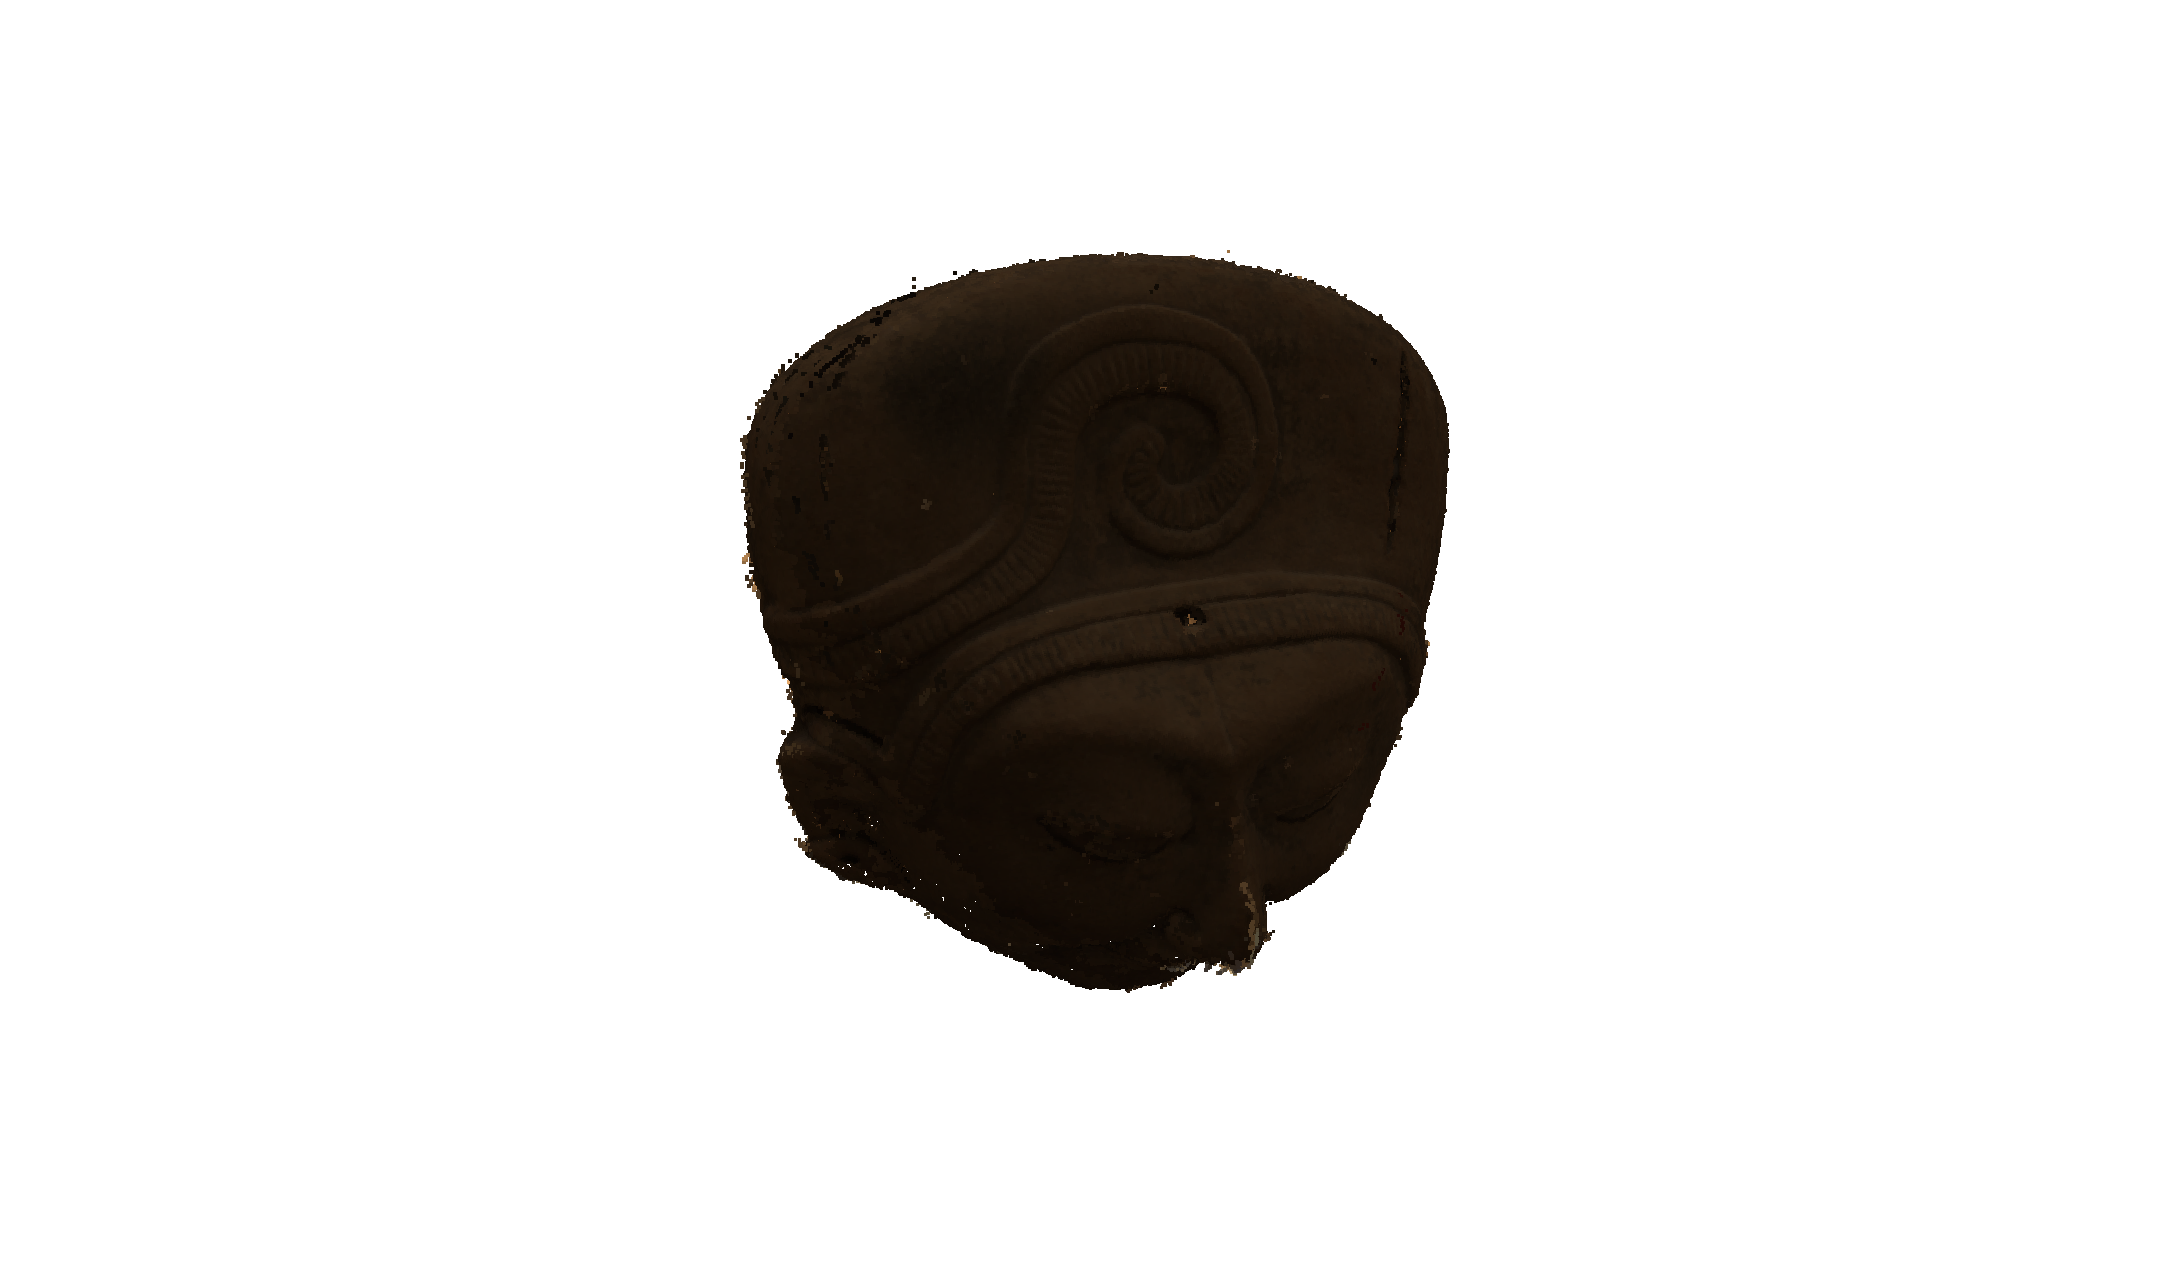
\includegraphics[scale=0.1]{image/静态点云示意图.png}
    }
    \hspace{0.1in}
    \subfloat[动态点云]{
        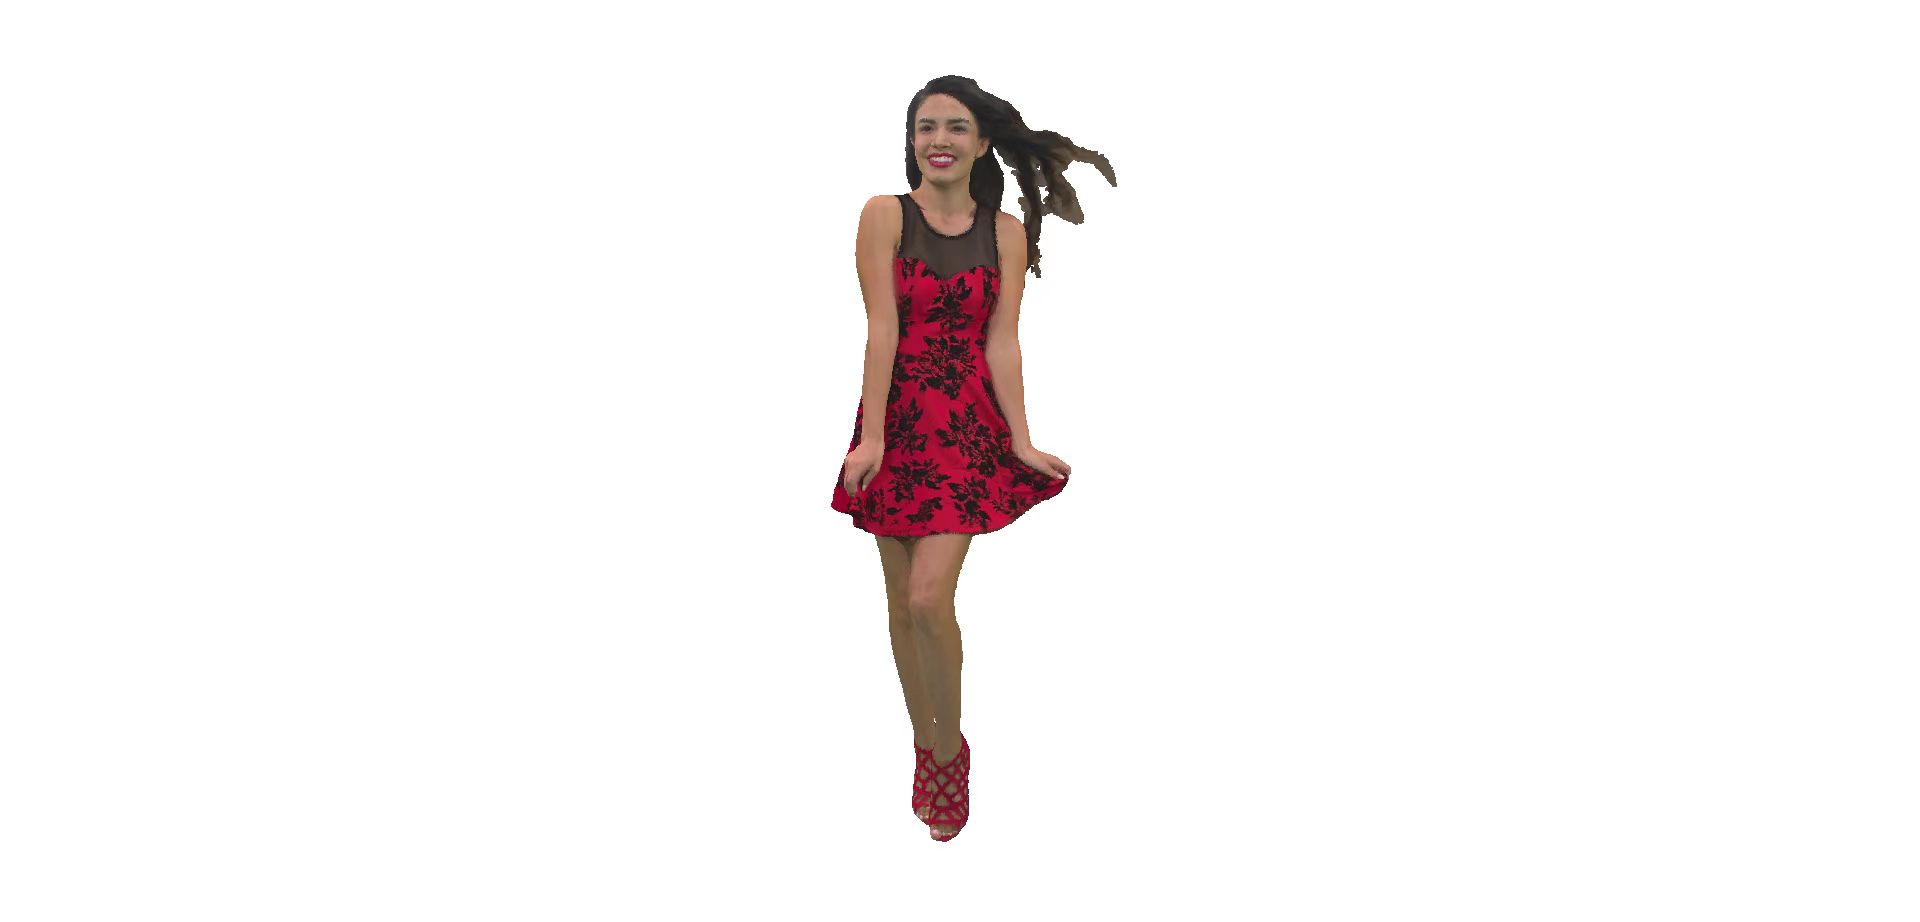
\includegraphics[scale=0.1]{image/动态点云示意图.jpg}
    }
    \hspace{0.1in}
    \subfloat[动态获取点云]{
        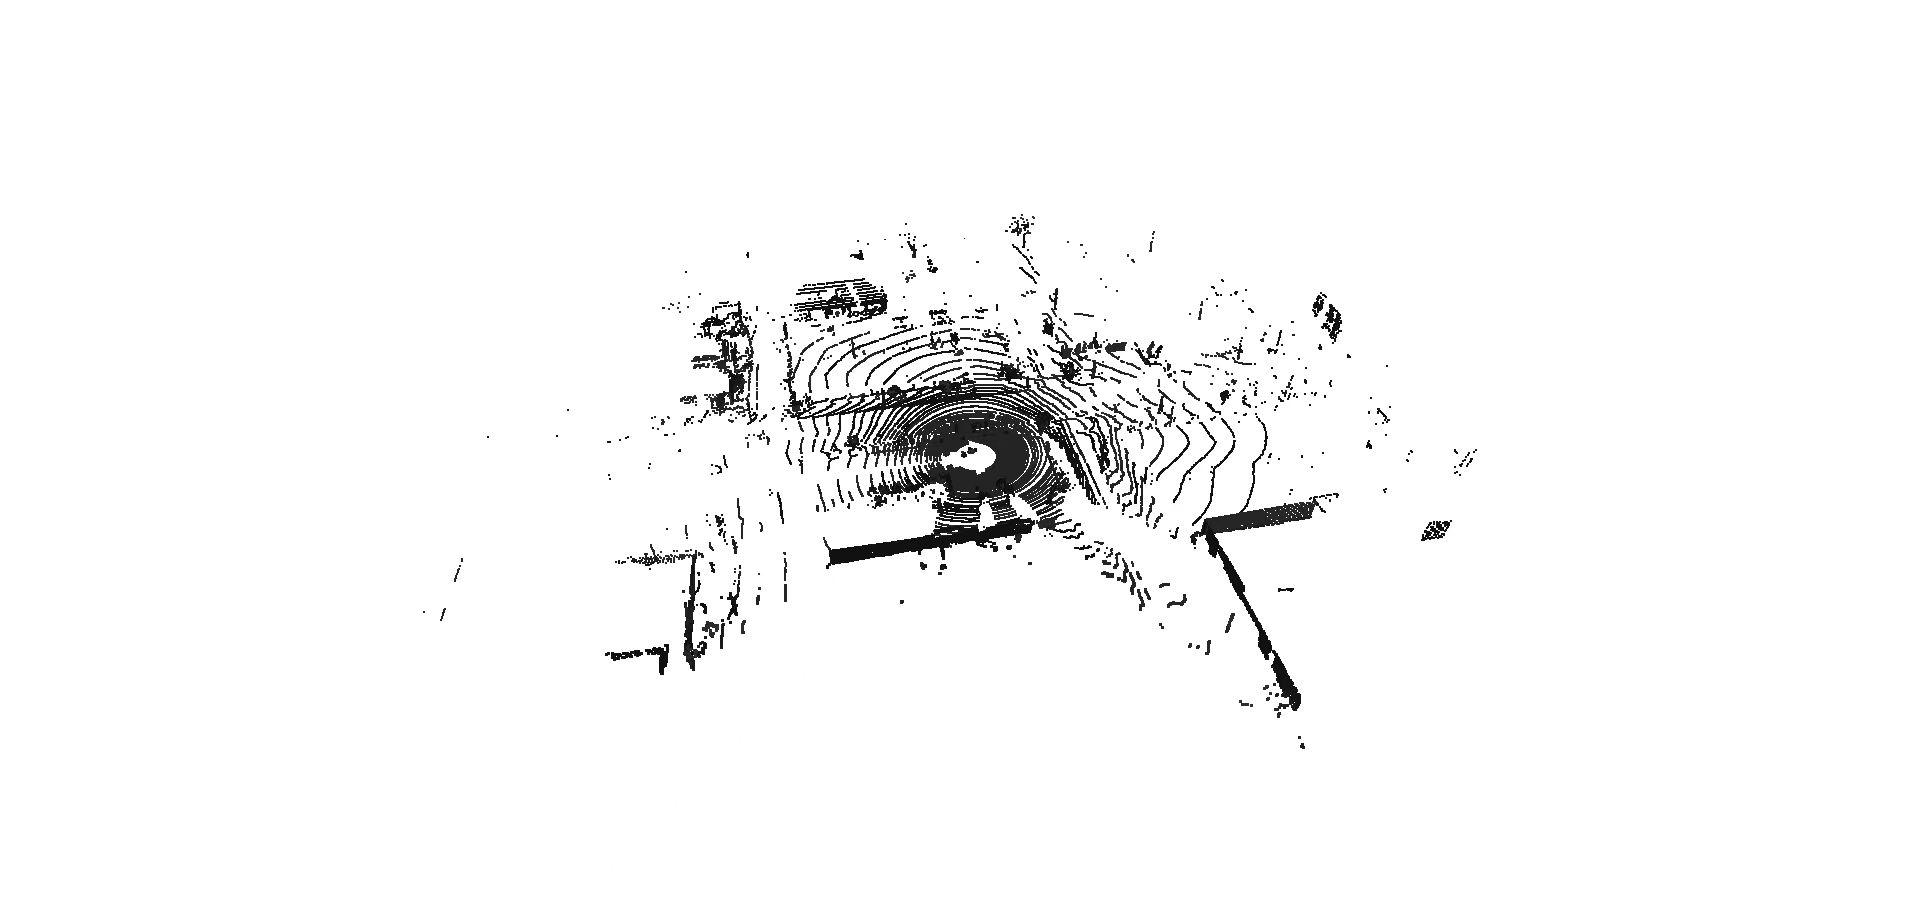
\includegraphics[scale=0.1]{image/动态获取点云.jpg}
    }
    \caption{三类点云示意图}
    \label{fig:三类点云示意图}
\end{figure}

点云获取技术的不断更新与发展,使得获得的点云模型精度不断提高,数量也急剧增大。越来越大的行业需求压力,促使着点云压缩技术的发展与标准化工作的展开。其中,MPEG提出的G-PCC标准主要针对静态点云和动态获取点云进行压缩,而V-PCC主要针对静态获取的动态点云进行压缩。

\section{GPCC框架}
本文主要对国际动态图像专家组MPEG提出的几何点云压缩(G-PCC)展开研究,该组织在为了方便测试和研究,推出了TMC13(Test Model for Category1 and Catgory3) 模型软件\cite{ref16},作为公开探索实验的参考平台。这一平台的具体编解码框架如图\ref{fig:编解码流程图}所示。从图中可以看出,不论是在编码端还是在解码端,几何信息和属性信息的编码都是分开进行的,以编码端为例:

几何信息编码首先对原始点云数据进行预处理,将点云几何信息进行坐标转换,使得变换后的点都在包围(BoundingBox)内再进行量化和重复点去除工作。然后对包围盒进行八叉树(Octree)划分,通过递归细分立方体的方法来构建八叉树结构。立方体每次八等分被划分成八个子立方体,之后再对非空的子立方体进行八等分,直到划分到体素大小为 1×1×1,使用占用码(occupancy code)表示一个立方体是否包含子立方体,1表示被占据,0表示不被占据,最后将占位信息送入熵编码器得到几何码流。Octree几何编码常用于TMC13,即动态获取点云,而针对表面稠密的静态点云(TMC1),Trisoup几何编码方式更具优势。Trisoup 是一种基于八叉树的几何编码方式,该方法先用八叉树划分到一定体素大小,然后应用 Trisoup 进行确定顶点和对顶点熵编码以达到压缩的目的,然后通过三角重建近似曲面进行解压缩,后续的属性编码也是基于重建后的点云进行。
\begin{figure}[htbp]
    %是可选项 h表示的是here在这里插入,t表示的是在页面的顶部插入
    \centering
    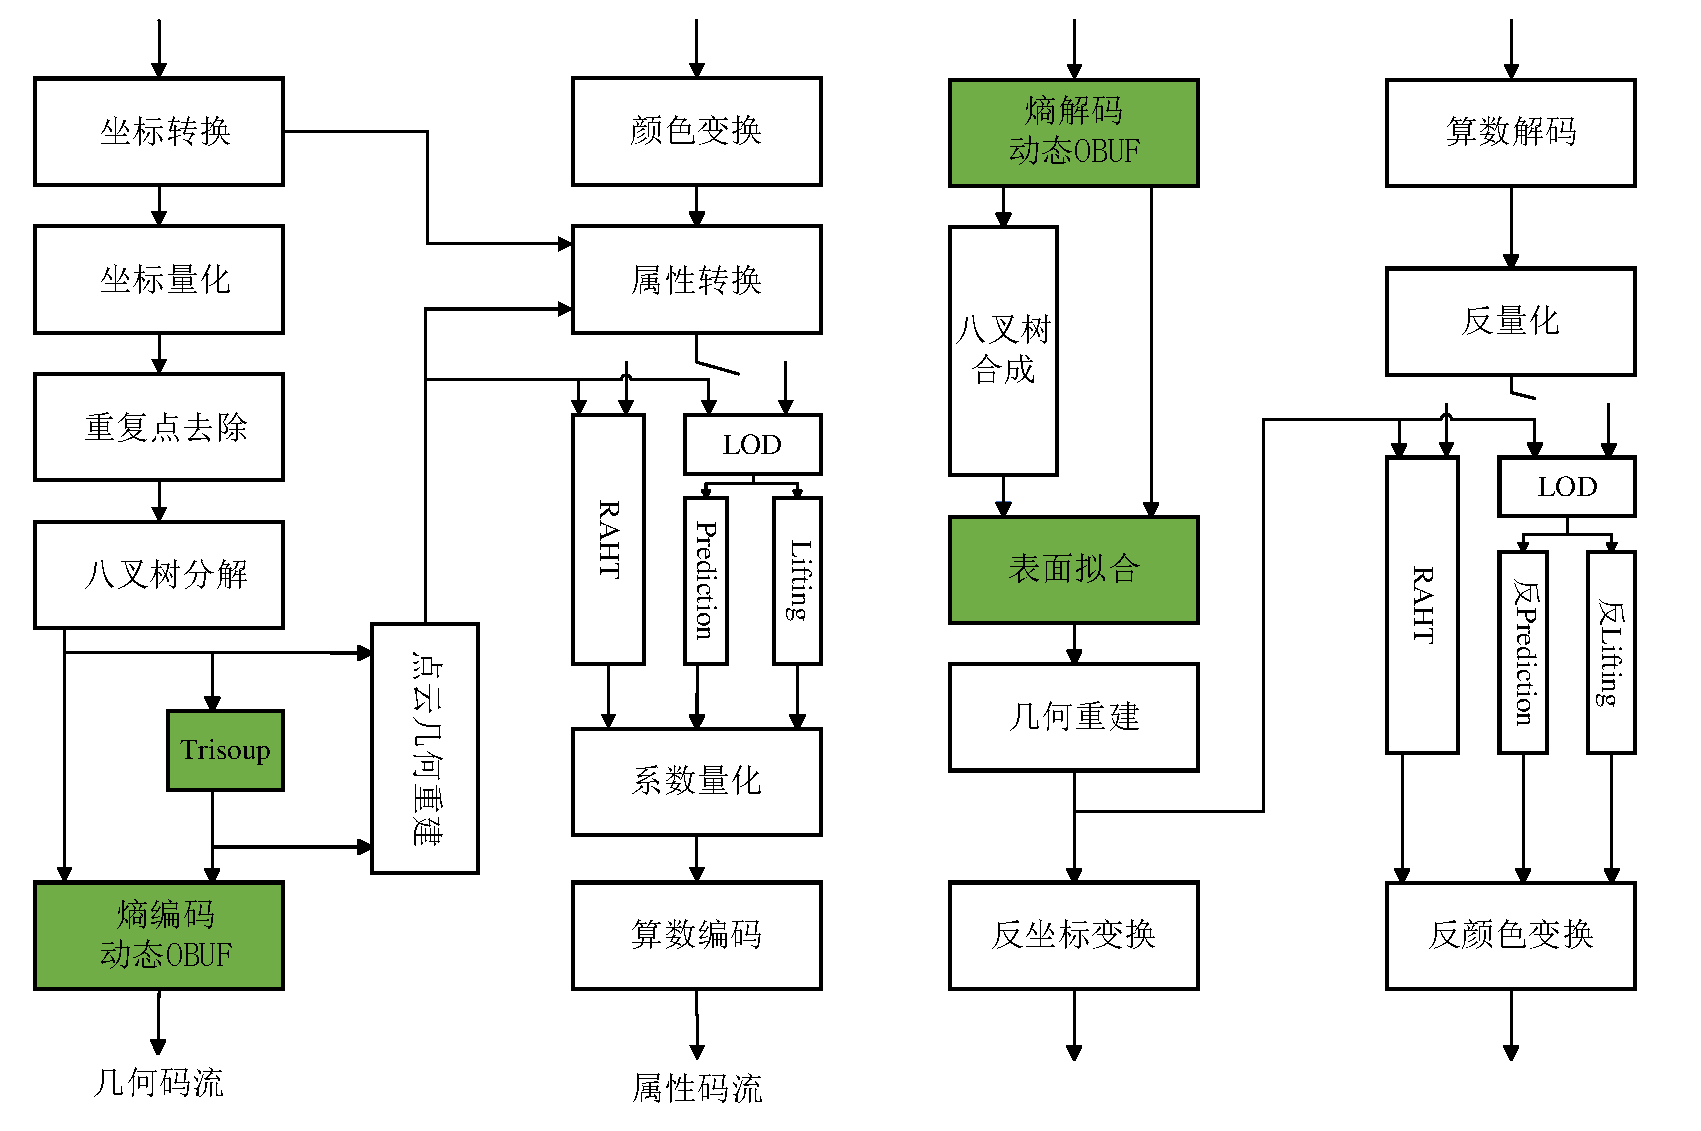
\includegraphics[scale=0.5]{image/编解码流程图ykv2.pdf}
    \caption{编解码流程图}
    \label{fig:编解码流程图}
\end{figure}

属性信息编码首先选择是否对对输入的属性信息进行颜色空间转换,目前TMC13 平台支持将颜色属性从 GBR 转换成 YUV 空间。当几何有损时,需要对点云进行属性转换,也就是对几何重建出来的点云重新赋予颜色信息。之后进行属性信息编码,根据不同的测试序列和条件选择适合的编码方式。接着将属性残差经过系数量化处理,最后通过熵编码得到最终的属性码流。

解码端对码流的处理流程即为编码端的逆过程。

另外,在现有的G-PCC标准中,使用Trisoup几何编码方式时,其熵编码过程用到了动态更新的最佳二值化技术(动态OBUF),相比于OBUf,该技术将上下文信息分为了主要信息和次要信息两部分,其中,主要信息用较少的bir位包含了上下文信息中最相关的部分,因此它不会变化;相反,次要信息会根据已使用的上下文信息能否将点云有效的区分开来进而来决定是否继续使用下一bit位上下文信息。这也是本文的主要研究内容。
\section{几何信息编码}
点云数据中一般存储着几何坐标、颜色、法线等信息。其中几何信息是必不可少的,它在物体的三维重建过程中起着决定性的作用。点云的几何形状通常用特定于应用程序的空间表示,其中点的位置可以用浮点数表示。因此,需要一个预处理步骤,将应用程序特定的空间转换为有限分辨率的内部空间。几何信息预处理的步骤一般包括:坐标转换,坐标量化、重复点去除。其具体过程如下:
\subsection{坐标转换}
获取到的原始点云中,各个点的位置通常是无规则的,并且通常由浮点数表示。因此,为了方便后续对几何信息进行压缩,首先将原始坐标系中点的位置坐标${\rm{X}}_{\rm{n}}^{orig}$用公式\ref{fig:公式1}转换为内部坐标系下的坐标${\rm{X}}_{\rm{n}}^{{\mathop{\rm int}}}$。
\begin{equation}
    {X_n} = ({\rm{X}}_n^{orig} - T)/s
    \label{fig:公式1}
\end{equation}

其中,$T=({t_x},{t_y},{t_z})$。参数$T$和$s$由包围盒$[0,{2^d})^3$中的点位置坐标${\rm{X}}_{\rm{n}}^{{\mathop{\rm int}}}$,$n = 1,...,N$(其中$ D $是非负整数参数)决定。

当采用八叉树几何编码时,$1/s$由$positionQuantizationScale$参数决定,$T = (\min x_n^{orig},\min y_n^{orig},\min z_n^{orig})$,d由公式\ref{fig:公式2}确定:
\begin{equation}
    d = Ceil(Lo{g_2}(Max(x_n^{{\mathop{\rm int}} },y_n^{{\mathop{\rm int}} },z_n^{{\mathop{\rm int}} },n = 1, \ldots ,{N_{orig}}) + 1))
    \label{fig:公式2}
\end{equation}
$[0,{2^d})^3$是最小的包围盒,所有的内部点位置坐标都在这个边长${2^d}$的立方体内。

当采用Trisoup几何编码时,s由参数$trisoupQuantizationBits$确定,T=[0,0,0],d由$trisoupNodeSizeLog2$参数确定。

\subsection{坐标量化}
在压缩之前,点位置坐标在内部被表示为$d$位非负整数。为了获得这些整数,点的位置坐标在内部坐标系中被量化取整。设${\rm{X}}_{\rm{n}}^{{\mathop{\rm int}}}$表示内部坐标系中的点位置坐标,量化公式如公式\ref{fig:公式3}所示:
\begin{equation}
    \left\{\begin{array}{l}
        x^{k}={round}\left(\frac{{x}^{\prime}}{Q S}\right) \\
        y^{k}={round}\left(\frac{y^{\prime}}{Q S}\right)   \\
        z^{k}={round}\left(\frac{{z}^{\prime}}{Q S}\right)
    \end{array}\right.
    \label{fig:公式3}
\end{equation}

其中,$QS$为量化步长,这里$round(s)$函数的功能是返回距$s$最近的整数,定义如下:
\begin{equation}
    {round}(s)=\left\{\begin{array}{cc}
        {int}(s+0.5)   & { if } s \geq 0 \\
        -{int}(-s+0.5) & { if } s<0
    \end{array}\right.
\end{equation}

\subsection{重复点去除}
量化之后会产生大量位置坐标相同的点,称为重复点。可以将具有相同量化坐标的重复点进行删除操作。坐标量化和删除重复点的过程称为体素化,也就是将一个体素内的所有点都量化到体素中心。如果一个体素内包含任意点云中的点,则称该体素被占用。

\subsection{八叉树编码}
八叉树是一种自顶向下的广度优先的树状数据结构,它可以用来存储表示三维空间物体和场景的几何信息。八叉树中的每个节点都代表着一个对应的正方体。对于每个非空的节点,可以将其继续划分为八个子节点,直至划分到叶子节点,即指定精度下的三维空间的最小单元。在对点云几何信息进行预处理之后,将对点云几何信息进行几何编码,首先将点云中各点的坐标转换为二进制表示。如果各点的几何位置用三维笛卡尔坐标表示为$(X,Y,Z)$,$n=0, …, N-1$,其中$N$是点云的总点数,那需要将其$X、Y、Z$坐标数值转化为$K$位比特表示的二进制数值:
\begin{equation}
    \left\{\begin{array}{l}
        X^{n}=\left(x_{K-1}^{n} x_{K-2}^{n} \cdots x_{1}^{n} x_{0}^{n}\right) \\
        Y^{n}=\left(y_{K-1}^{n} y_{K-2}^{n} \cdots y_{1}^{n} y_{0}^{n}\right) \\
        Z^{n}=\left(z_{K-1}^{n} z_{K-2}^{n} \cdots z_{1}^{n} z_{0}^{n}\right)
    \end{array}\right.
\end{equation}

按照莫顿码的生成规则,可以将点云中第$n$个点的三维几何坐标的三个维度上的$K$位比特表示的二进制数值逐位交叉排列,形成一个新的$3K$位比特表示的二进制数,也就是对应的莫顿码,表示如下:
\begin{equation}
    M^{n}=\left(x_{K-1}^{n} y_{K-1}^{n} z_{K-1}^{n}, x_{K-2}^{n} y_{K-2}^{n} z_{K-2}^{n}, \ldots x_{1}^{n} y_{1}^{n} z_{1}^{n}, x_{0}^{n} y_{0}^{n} z_{0}^{n}\right)
\end{equation}

将每三个比特用八进制数表示$
    m_{n}^{k}=\left(x_{n}^{k} x_{n}^{k} x_{n}^{k}\right), n=0,1, \ldots, N-1
$ , 则$K$点对应的莫顿码可以表示成:
\begin{equation}
    M^{n}=\left(m_{K-1}^{n} m_{K-2}^{n} \ldots m_{1}^{n} m_{0}^{n}\right)
\end{equation}

可以看出,每个点的坐标用莫顿码表示之后形成了$K$个八进制数排列组成的数据。由于八进制数的所有的取值情况可以表示8种情况,正好可以与八个子节点一一对应,而且随着$k$值的减小,每个八进制数都代表一层更深的八叉树划分。这样在每一层划分八叉树节点时,就可以很好的判断当前待划分的点要被划分至哪个子节点中。
\subsection{Trisoup几何编码}
Trisoup几何编码方式常用于TMC1,即静态获取且表面密集的点云。在几何信息编码中,常常先用八叉树划分到一定层次,然后应用Trisoup进行确定顶点和对顶点熵编码以达到压缩的目的,然后通过三角重建近似曲面进行解压缩,也就是说Trisoup是一种基于八叉树的几何编码方式。但是在当前几何信息编码标准测试环境中,对于每一个点云文件在进行编码时八叉树应该划分到哪一层都有固定的值,由参数$trisoupNodeSizeLog2$确定。

Trisoup几何编码主要分四个步骤进行:
\begin{figure}[h]
    %是可选项 h表示的是here在这里插入,t表示的是在页面的顶部插入
    \centering
    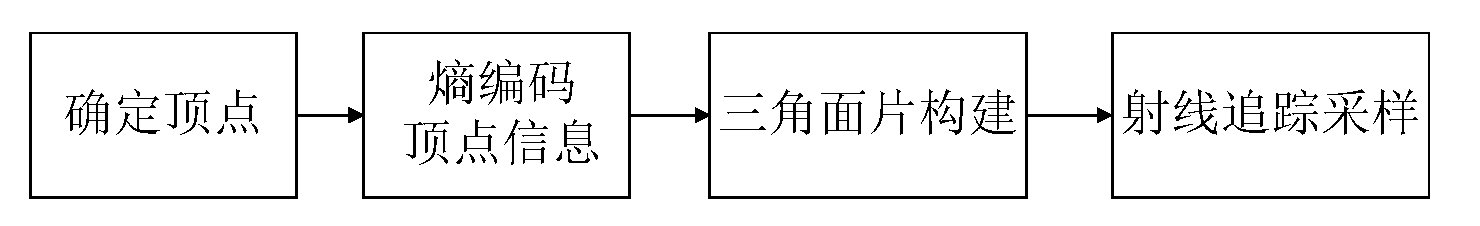
\includegraphics[scale=0.5]{image/Trisoup流程图_crop.pdf}
    \caption{Trisoup流程图}
\end{figure}

1、确定顶点。几何图形在每个块中表示为一个至多与块的每条边相交一次的曲面。由于一个块有12条边,所以在一个块中最多可以有12个这样的交点。每一个这样的交点称为顶点。当且仅当共享该边的所有块中与该边相邻的块中至少有一个已占用的体素时,才能检测到沿该边的顶点。检测到的顶点沿边的位置是共享该边的所有块中,所有与该边相邻的体素沿边的顶点的平均位置。

2、熵编码顶点信息。顶点信息包含两部分:一个是标识信息,即标识所有被占据的叶子节点中哪些边上有顶点,也称为边被占据,被占据标识为 1,不被占据标识为 0;另一个是顶点位置信息,对于每个被占据的边,顶点位置信息被量化为 2bit。最后利用算数编码器对标识信息与顶点位置信息进行熵编码。

3、三角面片构建。根据三角形投影面积大小确定主导轴、求出质心坐标以及质心偏移量、根据方位角信息对顶点进行排序。最后将顶点与质心组合,构建三角面片。如图\ref{fig:三角面片构建}所示。
\begin{figure}[h]
    %是可选项 h表示的是here在这里插入,t表示的是在页面的顶部插入
    \centering
    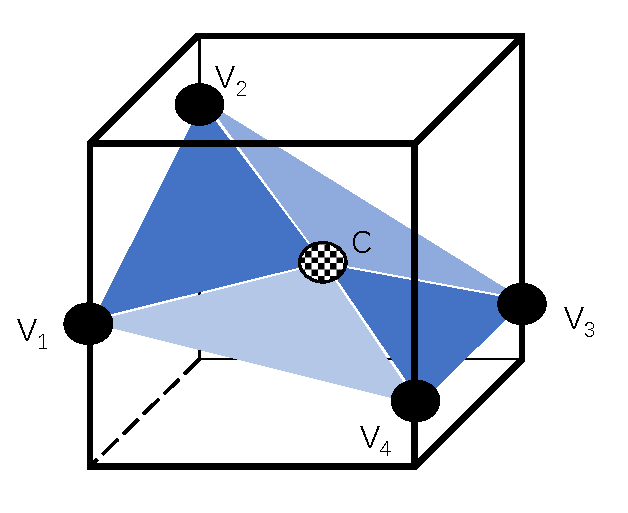
\includegraphics[scale=0.5]{image/三角面片构建v2.pdf}
    \caption{三角面片构建示意图}
    \label{fig:三角面片构建}
\end{figure}

4、射线追踪采样。以三角面片在主轴方向上的投影面为射线起点,射线追踪的间隔由高层语法元素决定,同时会根据重建后的点云数量改变间隔大小。射线追踪采样的核心是利用Muller-Trumbore算法\cite{ref22},判定射线是否与三角面片有交点,产生的交点便是重建点云。如图\ref{fig:射线追踪采样}所示。
\begin{figure}[htbp]
    %是可选项 h表示的是here在这里插入,t表示的是在页面的顶部插入
    \centering
    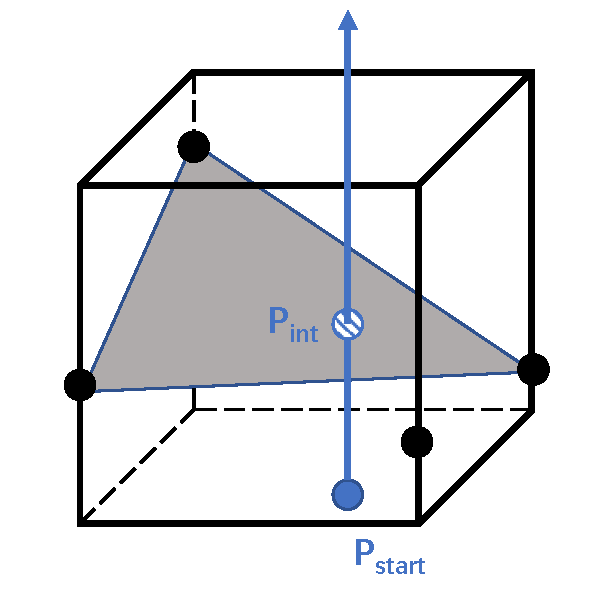
\includegraphics[scale=0.5]{image/射线追踪v2.pdf}
    \caption{射线追踪采样示意图}
    \label{fig:射线追踪采样}
\end{figure}

为了使熵编码更加的高效,编码得到的bit流更小,熵编码顶点信息过程中使用了动态OBUF。顶点标识信息与顶点位置信息分开编码,用到了两组不同的上下文信息,同时上下文信息又分为主要信息与次要信息:主要信息用较少的bit数承载了绝大部分相关性信息,去除该相关性以后再进行熵编码,码流显然会减少;次要信息的动态使用则是动态OBUF的特点所在,它会根据熵编码输出的值更新LUT以及上下文使用数量。
\subsection{动态OBUF}
\label{动态OBUF}
在MPEG给出的TMC13v20参考代码中,采用Trisoup几何编码方式时,最后将顶点的标识信息、顶点的位置信息进行熵编码时,采用的是基于动态更新的最佳二值化的熵编码器(动态OBUF),其编码框架如图\ref{fig:动态OBUF流程图}所示,动态OBUF的基本工作流程与OBUF一致,它只是新加入了上下文的动态缩减过程,以达到使编码当前符号的概率模型更加迅速的趋于信源概率模型的目的。
\begin{figure}[h]
    %是可选项 h表示的是here在这里插入,t表示的是在页面的顶部插入
    \centering
    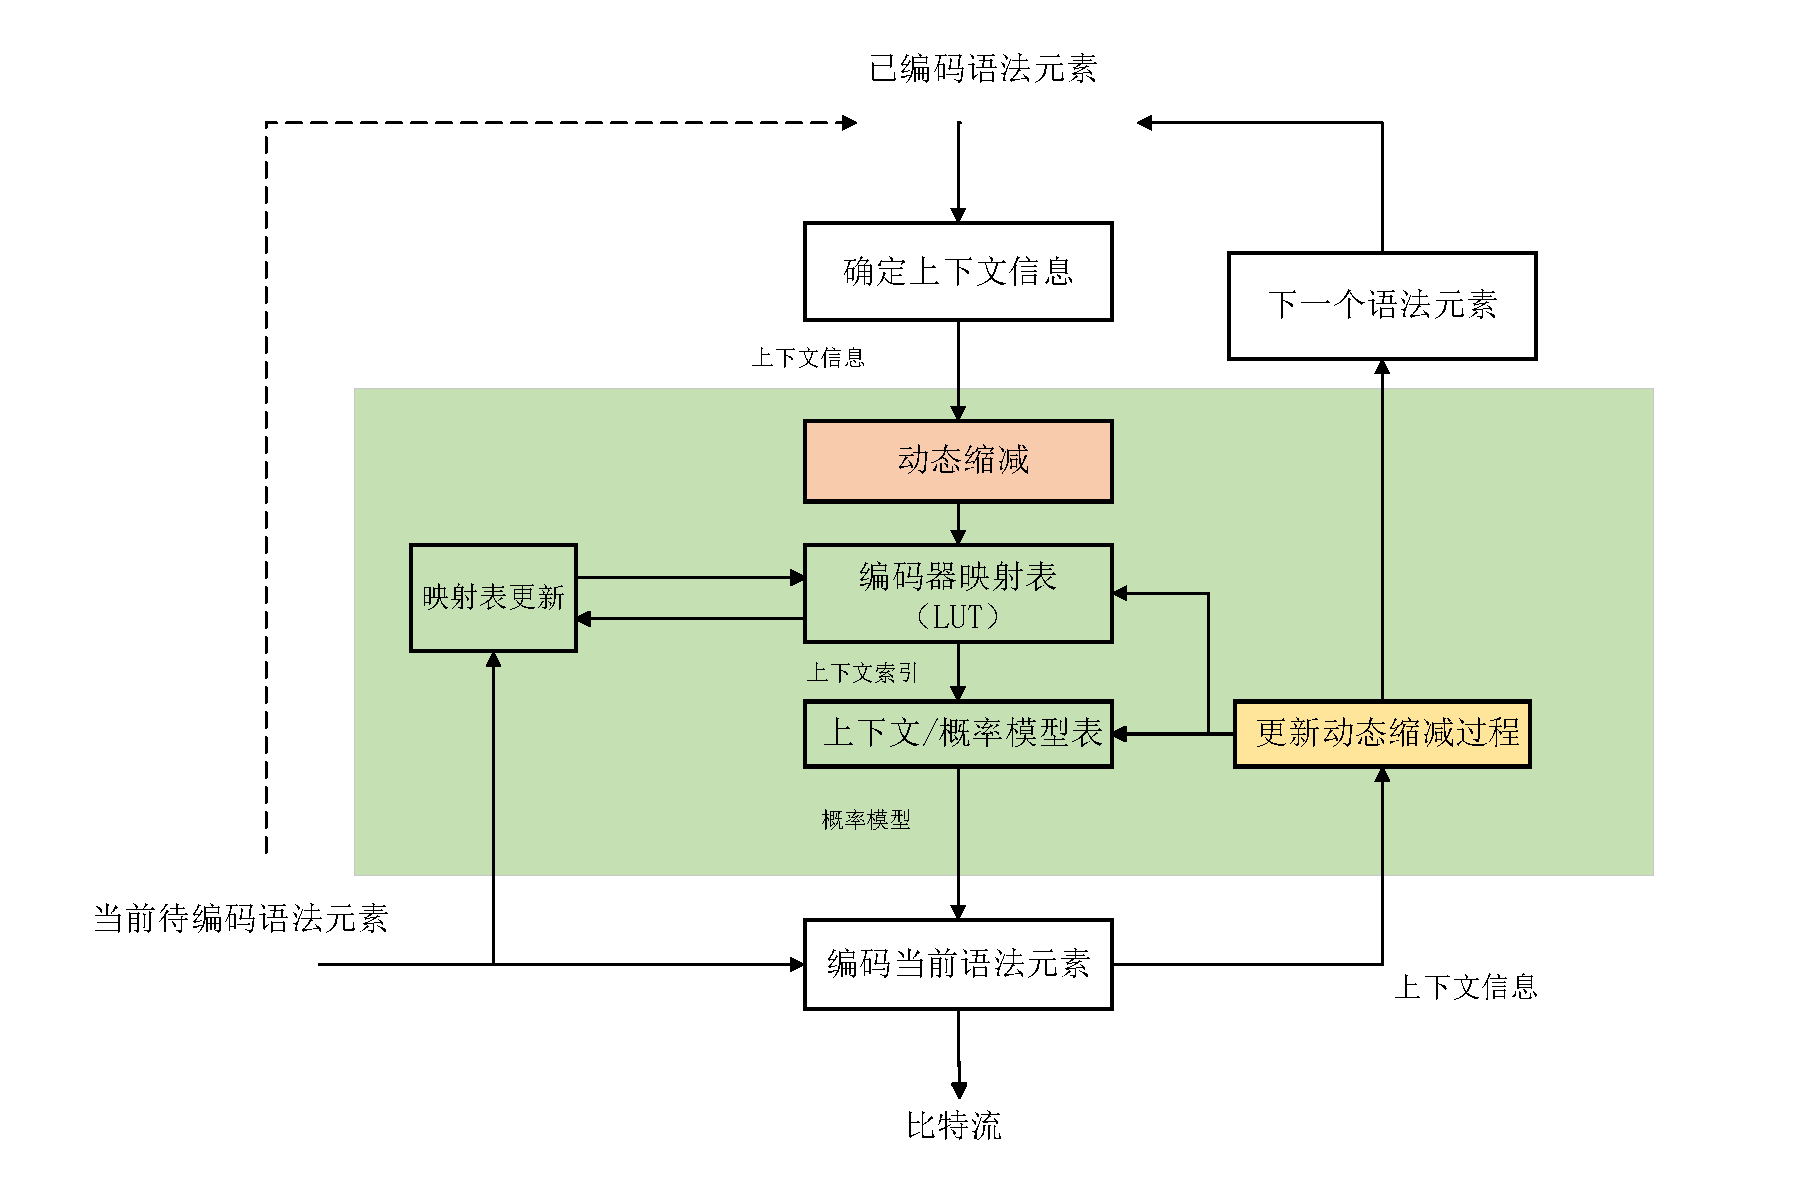
\includegraphics[scale=0.4]{image/动态OBUF流程图ykv2.pdf}
    \caption{动态OBUF流程图}
    \label{fig:动态OBUF流程图}
\end{figure}

动态OBUF相比于OBUF不同之处在于它将上下文信息分为了主要信息(Primary Information)和次要信息(Second Information),其中主要信息以较少的bit数承载着强相关的上下文信息,主要信息是不会随着熵编码的不断进行而减少的;次要信息的使用是动态OBUF的特点所在,图中标识的部分具体细节如图\ref{fig:dynamicreduction示意图}与\ref{fig:updatedynamicreduction示意图}所示。
\begin{figure}[h]
    %是可选项 h表示的是here在这里插入,t表示的是在页面的顶部插入
    \centering
    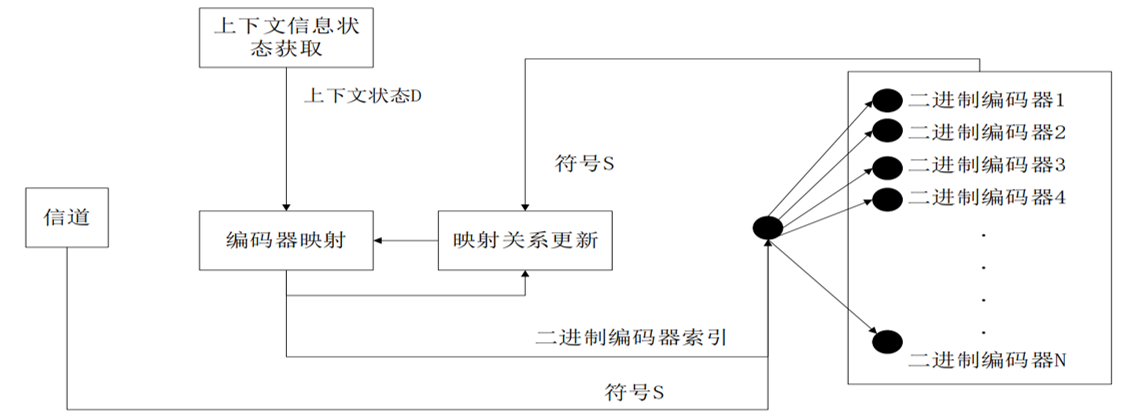
\includegraphics[scale=0.5]{image/OBUF工作原理图.png}
    \caption{OBUF工作原理图}
\end{figure}

动态减少是针对次要信息进行的,整个动态减少的过程主要由计数器N(i1,i2’)和决定次要信息使用bit位数的K两个参数控制,其中N(i1,i2’)是记录整个编码过程访问当前上下文的次数,当计数器超过一定的阈值$th$时,如图\ref{fig:updatedynamicreduction示意图}所示,首先DRn将会更新为DRn+1,这同样与熵编码器的索引表(LUT)相适应,最后还需要将计数器置零。另外,次要信息可以表示为${\rm{i}}2 = {\beta _{_1}}{\beta _2} \ldots {\beta _{\rm{k}}}$,通过更新K值,再对次要信息进行移位操作,便可达到动态更新次要信息的效果。

这样设计的目的在于,在编码初期,熵编码只会使用到很少的次要信息甚至仅使用主要信息就可以高效率的将待编码语法元素编码完成,因此大大节省了熵编码的bit流,提高了编码效率。
\begin{figure}[htb]
    %是可选项 h表示的是here在这里插入,t表示的是在页面的顶部插入
    \centering
    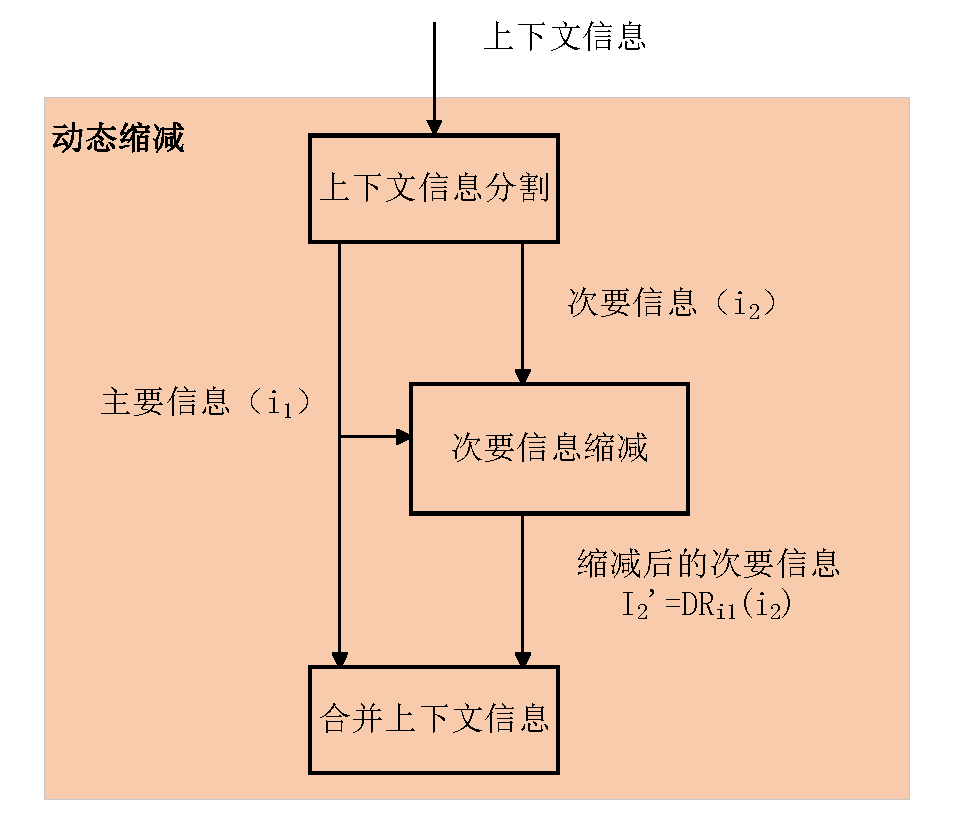
\includegraphics[scale=0.4]{image/动态缩减_crop.pdf}
    \caption{dynamicreduction示意图}
    \label{fig:dynamicreduction示意图}
\end{figure}
\begin{figure}[htb]
    %是可选项 h表示的是here在这里插入,t表示的是在页面的顶部插入
    \centering
    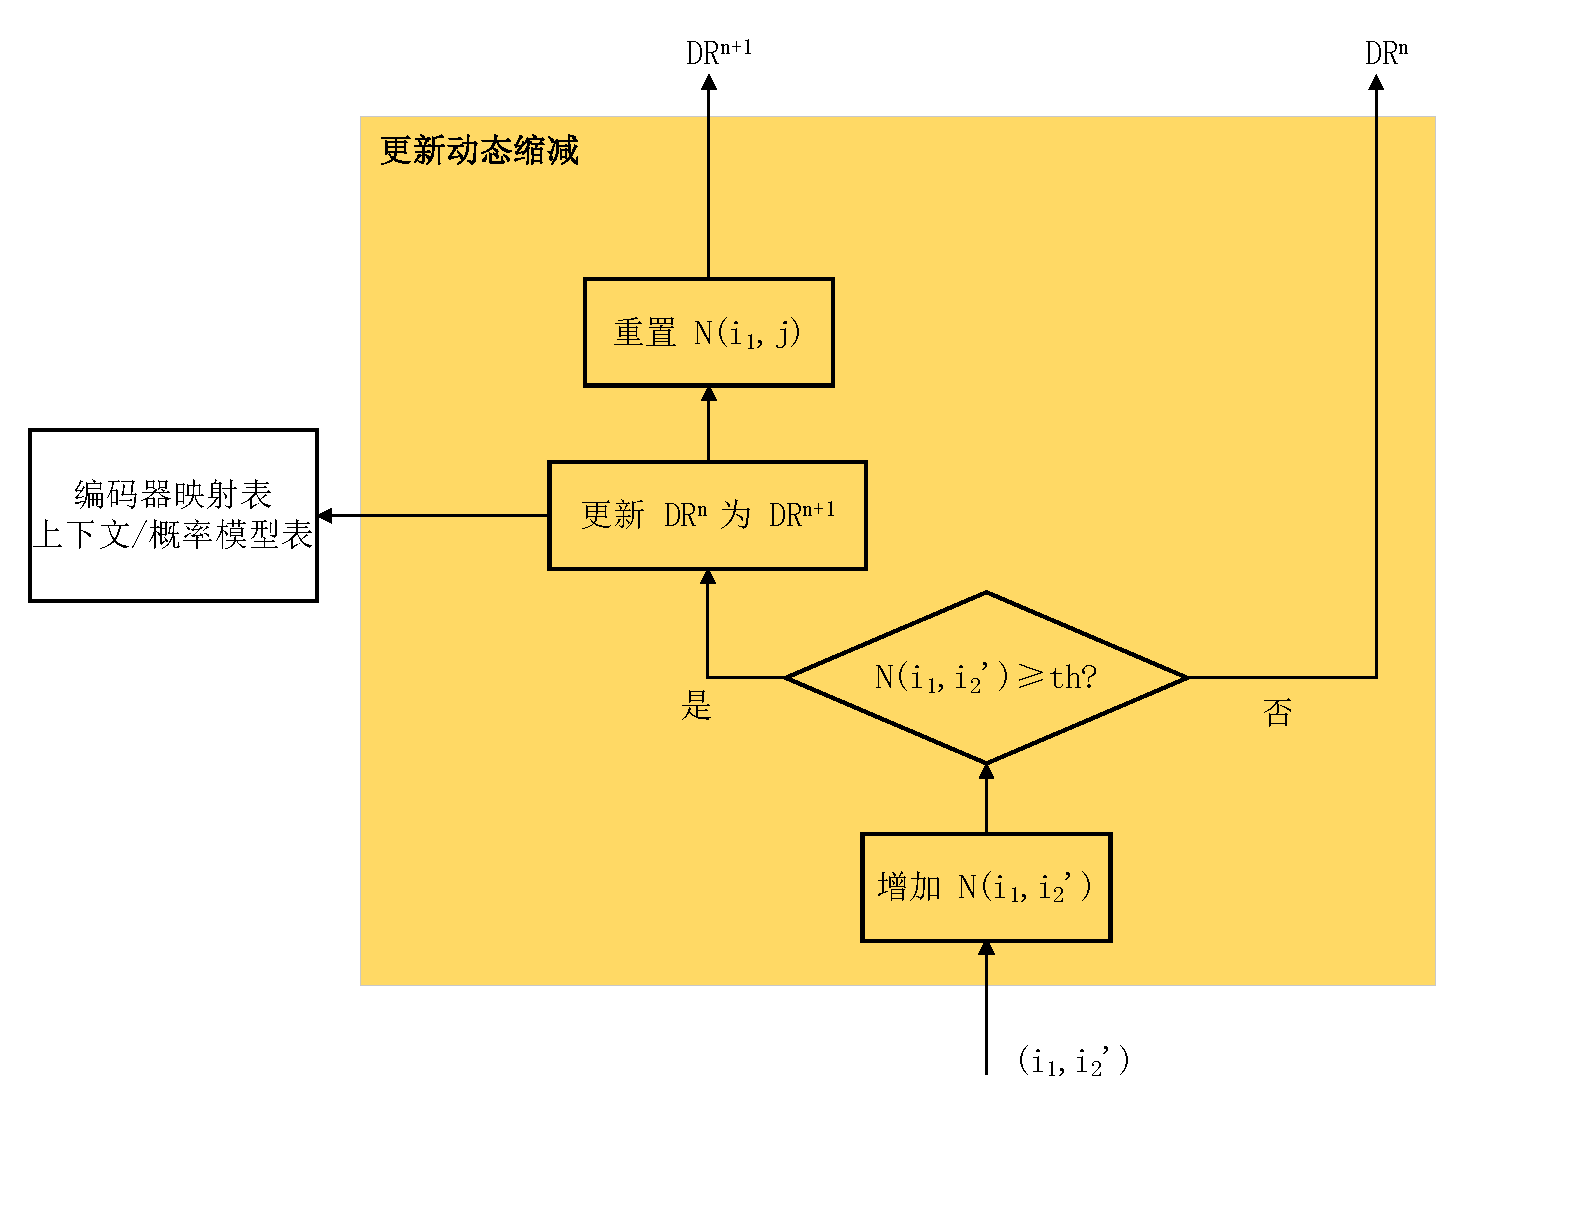
\includegraphics[scale=0.3]{image/更新动态OBUF_crop.pdf}
    \caption{updatedynamicreduction示意图}
    \label{fig:updatedynamicreduction示意图}
\end{figure}

\section{属性信息编码}
\label{sec:organization}
由图\ref{fig:编解码流程图}可以直观的看出,G-PCC主要包括两种属性变换编码方法,第一种是基于插值的带更新/提升的分层最近邻预测(Lifting Transform),第二种是区域自适应分层变换(RAHT)。其中,与Trisoup几何编码方法配合使用的主要是第二种。另外,这两种变换编码方式通常用于第一类点云数据。
\subsection{颜色变换}
G-PCC提供了颜色空间转换的功能,方便在不同场景下,应用合适的颜色空间。例如从RGB到YUV的颜色空间转换,具体公式如下所示:
\begin{equation}
    \left\{\begin{array}{c}
        Y=0.2126 \times R+0.7152 \times G+0.0722 \times B       \\
        U=-0.114572 \times R-0.385428 \times G+0.5 \times B+128 \\
        V=0.5 \times R-0.454153 \times G-0.045847 \times B+128
    \end{array}\right.
\end{equation}

转换的逆过程有:
\begin{equation}
    \left\{\begin{array}{c}
        R=Y+1.5748 \times(V-128)                        \\
        G=Y-0.18733 \times(U-128)-0.46813 \times(V-128) \\
        B=Y+1.85563 \times(U-128)
    \end{array}\right.
\end{equation}

其中,在整个颜色转换的过程中,使用的所有数据都是浮点型的,但是标准定义的输出结果统一转换为$unit8_t$格式,因此经过颜色空间转换后,颜色信息会产生一定的偏差,这也就限定了颜色空间转换只适应于属性有损条件下进行。

\subsection{属性转换}
进行属性信息编码前,因为当几何编码是有损时,重建出来的点云坐标位置与原始几何坐标有偏差,所以重建的点云没有属性信息,这个时候需要将原始的属性信息进行属性转换,为点云重新着色,同时需要保证属性失真最小。目前,在TMC13中,可以通过计算原始点云值多个近邻的距离加权平均数来实现属性转换。具体的属性转换过程如下:

1、为重建点云$(\widehat{X}_{i})_{i=0 \ldots  N_{r e c}-1}$建立起KD-Tree,将三个维度中的最长边方向作为划分主轴,其次基于划分主轴方向对重建点云进行划分。然后遍历原始点云的每个点,在重建点云KD-Tree结构中进行最近邻居点$Ref1$查找。由于是遍历的原始点云,因此最近邻居点会出现两种情况,一种是在重建点云中某个点作为原始点云中多个点的最近邻居点;第二种是原始点云中所有点都不会将某个重建点作为最近邻居点。

2、对原始点云$(X_{i})_{i=0\cdots N-1}$建立起KD-Tree,将三个维度中的最长边方向作为划分主轴,其次基于划分主轴方向对重建点云进行划分。然后遍历重建点云中的每个点,在原始点云KD-Tree结构中进行最近邻居点$Ref2$查找。但是由于是遍历重建点云的每一个点,每重建点都会找到一个原始点云作为其最近邻居。

3、首先判断$Ref1$集合是否为空,如果为空,则当前重建点的属性信息由相应索引的$Ref2$得到,否则当前重建点的属性由公式可得:
\begin{equation}
    \hat{A}_{i}=\frac{1}{num} \sum_{k=1}^{Ref(i)} A_{k}(i)
\end{equation}

\subsection{RAHT变换编码}
在八叉树划分的结构下,相邻节点里的属性值可能会比较相近,即这些属性信号的交流分量几乎为0,能量主要集中在直流分量上,通过变换将原始属性值转换成对应的AC,DC系数,就可以更好的对信号进行压缩去冗余。在GPCC中RATH变换\cite{ref21}主要过程如下:

1.构建和解析树

开始构建树时,需要对点云中所有的点按照莫顿序逐次进行扫描,通过莫顿码右移,不断将点云序列中的点进行合并,从而逐层构建树。在构建树的过程中,每个点的初始权重$weight_{org}$设置为1,初始颜色属性为$Attr_{org}$,每当两个点进行合并时,合并后点的属性值和权重分别为:
\begin{equation}
    Attr_s=Attr_{org1}+Attr_{org2}
\end{equation}
\begin{equation}
    weight_s=weight_{org1}+wieght_{org2}
\end{equation}

不断进行莫顿码右移和迭代,直至整个点云序列中只有一个点。解析树的过程是构建树的相反过程,基本规则相同。

2.预测和变换

由于最高级父块处于树的顶部位置,并没有可以用于参考从而进行预测的父块或者祖父块,因此第n-1到n-4层不进行预测,当预测标识开启时,除第一级父块外的其余层都会进行预测。通过occupancy标记当前父节点中8个子节点的占用情况。通过父级块对当前块进行预测,首先要寻找当前块的父块的19(1+6+12)个邻居节点,其中,1为邻居节点是当前块的父节点,6为与父节点共面的邻居节点,12为与父节点共线的邻居节点,但这19个邻居节点不一定总是被占据,所以需要对邻居节点进行标识,用“1”表示当前子节点被占据,用0表示当前子节点不被占据,邻居节点示意图如 \ref{fig:邻居节点的示意图} 所示:
\begin{figure}[h]
    %是可选项 h表示的是here在这里插入,t表示的是在页面的顶部插入
    \centering
    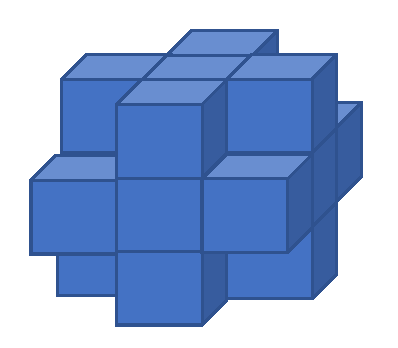
\includegraphics[scale=0.7]{image/邻居节点示意图v2.pdf}
    \caption{邻居节点的示意图}
    \label{fig:邻居节点的示意图}
\end{figure}

查找完邻居节点后,就需要对子节点进行预测。不同类型的邻居节点,在预测中所占的权重是不一样的。首先是父节点对子节点预测效果最好,其次是共面的父邻居节点,再者是共线的父邻居节点。因此在设置预测权重时,权重值依次递减。

对属性信息和预测的属性信息进行RAHT变换,根据构造的树的结构,从最高层开始,每三层进行RAHT变换,其中每个父块作为变换块来依次进行RAHT变换。
如果进行在该层进行预测,则需要对属性信息和预测属性信息都进行RAHT变换;如果不进行预测,则只需要对属性信息进行RAHT变换。用$w_1$和$w_2$分别表示两个待变换块包含的点数,用$c_1$和$c_2$表示两个待变换块的属性值,则RATH变换公式如\ref{fig:RAHT公式1}和\ref{fig:RAHT公式2}所示:
\begin{equation}
    \mathrm{RAHT}\left(w_{1}, w_{2}\right)=\frac{1}{\sqrt{w_{1}+w_{2}}}\left[\begin{array}{cc}
            \sqrt{w_{1}}  & \sqrt{w_{2}} \\
            -\sqrt{w_{2}} & \sqrt{w_{1}}
        \end{array}\right]
    \label{fig:RAHT公式1}
\end{equation}

\begin{equation}
    \left[\begin{array}{l}
            D C \\
            A C
        \end{array}\right]=\mathrm{RAHT}\left(w_{1}, w_{2}\right)\left[\begin{array}{l}
            c_{1} \\
            c_{2}
        \end{array}\right]
    \label{fig:RAHT公式2}
\end{equation}
其中DC系数为属性的加权平均值,AC系数为相邻两点的属性残差。计算AC系数的残差,计算公式如\ref{fig:RAHT公式3}所示:
\begin{equation}
    Attr _ {res }=  AttrCoff_{org} -  AttrCoff_{pred }
    \label{fig:RAHT公式3}
\end{equation}

若当前层不进行预测,则直接对属性信息变换系数进行量化和熵编码。若当前层需要进行预测时,对上述步骤得到的AC系数的残差进行量化和熵编码。

\subsection{Lifting预测变换编码}
该方法利用点云中已编码点的属性值对待编码点进行预测,从而得到待编码点的属性预测值,并将待编码点的真实属性值与预测值相减得到预测残差,以达到去除空域冗余的目的。基于莫顿码排序选取预测点,一定程度上反映了空间近邻的相关性,但是由于存在空间跳跃点等情况,预测效果并不是很好。因此引入了LOD (Level Of Detail) 划分技术\cite{ref20},也就是将点云划分成不同的层次结构,利用层次结构对属性进行有效预测。

LOD 划分有三种方法,包括基于距离的 LOD 划分、基于采样率的 LOD 划和基于八叉树的 LOD 划分。如图 \ref{fig:10} 所示,基于距离的 LOD 划分适用于稠密均匀的点云,如 cat1类型;基于采样率的 LOD 划分适用于分布稀疏不均匀的点云,如 cat3-frame 和 cat3-fused 类型;基于八叉树的 LOD 划分适用于 scalable 情况,对齐几何和属性的点数,使其与几何八叉树结构对齐。

Lifting 变换编码是一种依赖于多层LOD的属性编码方式,也就是将点云划分成不同的层次结构,利用层次结构对属性进行有效预测。其主要包含了分割、预测、更新三个部分,如图\ref{fig:提升变换流程图}所示。
\begin{figure}[h]
    %是可选项 h表示的是here在这里插入,t表示的是在页面的顶部插入
    \centering
    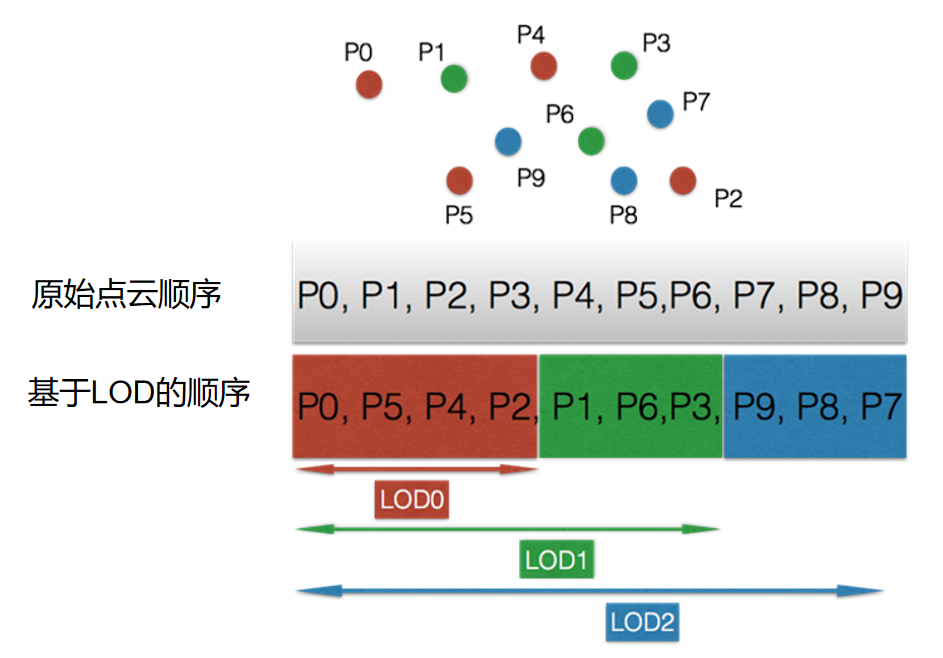
\includegraphics[scale=0.3]{image/LOD.png}
    \caption{基于距离的LOD划分示意图}
    \label{fig:10}
\end{figure}

\begin{figure}[h]
    %是可选项 h表示的是here在这里插入,t表示的是在页面的顶部插入
    \centering
    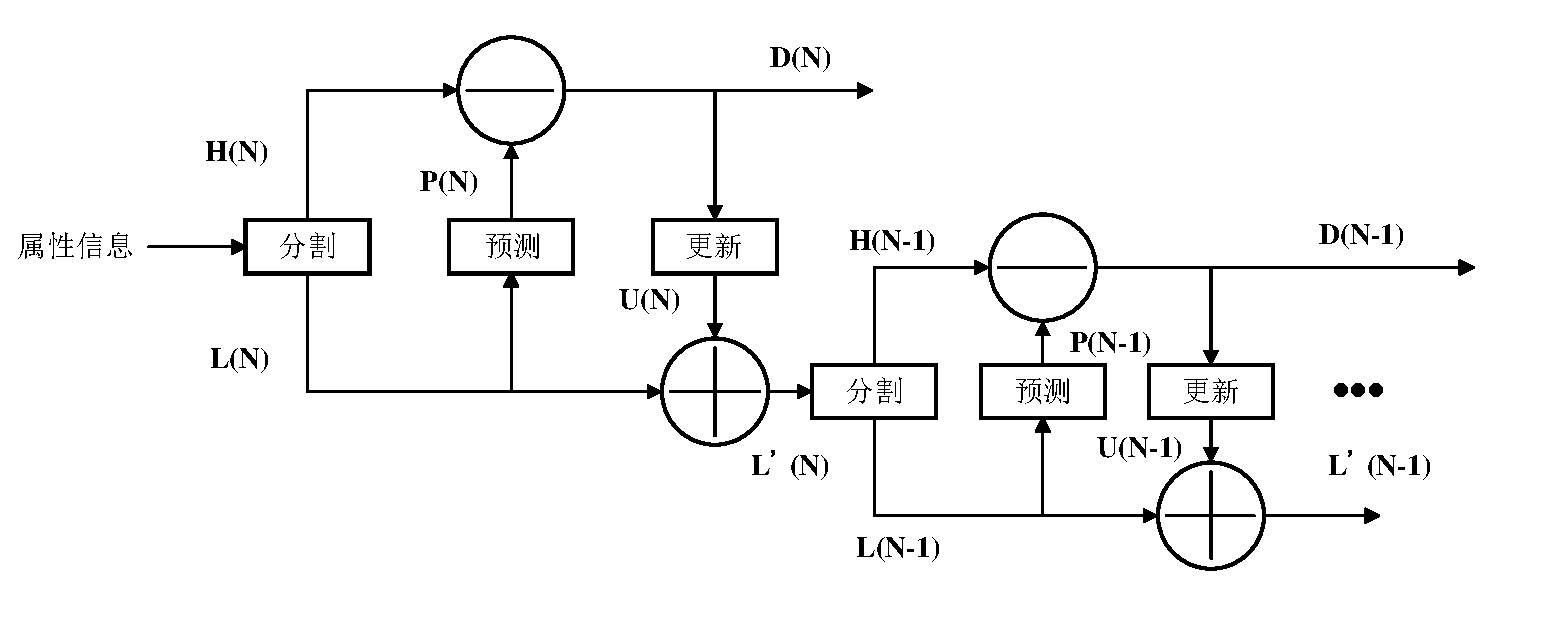
\includegraphics[scale=0.5]{image/提升变换流程图v2.pdf}
    \caption{LOD划分示意图}
    \label{fig:提升变换流程图}
\end{figure}

其中,$H(N)$表示高层次点云是与细化层相关的属性集,$L(N)$表示低层次点云是与$LOD(N)$相关的属性集,$D(N)$表示预测残差。

Lifting变换建立在分层预测的基础上,引入了权重更新和自适应量化的概念。低层 LOD 层被频繁的用来预测高层 LOD 层中的点,所以更新量化权重的目的是给低层 LOD 层点云提升一定的权重值来表征其重要性,使其影响更大,量化损失更小,预测结果更准确。Lifting 变换的关键在于预测和更新算法。预测算法得到的预测残差是变换过程中的高频分量,而通过更新算子来提升的属性信息是输入信号的低频分量。低频分量表征了点云属性的基本特征,反映出点云属性的整体情况,高频分量表征了点云属性的更多细节特征。Lifting 变换运算时间短,占用存储少,可准确地将点云属性划分为低频和高频两个部分,具有良好的压缩性能和重建效果

\section{评价标准}
\label{sec:suborganization}
评价一个点云压缩算法的性能好坏一般从三个方面出发:

1、编解码前后点云失真情况,具体又细分为几何失真与属性失真。两部分的失真计算都是基于对应点的,几何失真计算的是几何距离的失真,属性失真计算的是属性数值的失真。其中对应点就是原始点云的点在重建点云中的最近邻居点或者重建点云中的点在原始点云中的最近邻居点。

2、编码后比特流的大小。比特流大小可以通过 Bpip(bits per input point,即平均每个输入点所用比特数)来衡量,Bpip 越小,压缩性能越好。

3、编解码点云的时间复杂度。时间复杂度可以通过编解码过程耗费的时间来衡量,时间越短,压缩性能越好。

在无损压缩情况下,不存在点云的失真,只要考后两个方面来衡量性能。在有损压缩的情况下,点云的失真程度也是重要的考量,在衡量性能时三个方面都要考虑。在实际评估过程中,可从 rate 模式和 PSNR 模式两方面进行比较。BD-rate 为负值时,表示相同 PSNR 的条件下,码率减小,性能提升;BD-PSNR为负值时,表示相同码率的条件下,PSNR 增大,性能提升。


\ifx\allfiles\undefined
\end{document}
\fi
%%% Local Variables:
%%% TeX-master: "thesis-doctor.tex"
%%% End:
%% ----------------------------------------------------------------------
%%% END OF FILE 
%% ----------------------------------------------------------------------